\documentclass{article}
\usepackage[utf8]{inputenc}
\usepackage{amsmath,amssymb}
\usepackage{enumitem}
\usepackage{graphicx,tikz}
\usepackage{geometry}
\usepackage{hyperref}

\geometry{margin=1in}
\pagestyle{empty}
\setlength{\parindent}{0pt}
\setlength{\parskip}{0.5em}

\newcommand{\code}[1]{{\fontfamily{pcr}\selectfont #1}}
\newcommand{\abs}[1]{\left|#1\right|}
\newcommand{\srs}[1]{\{#1\}_1^\infty}
\newcommand{\floor}[1]{\left\lfloor#1\right\rfloor}
\newcommand{\ceil}[1]{\left\lceil#1\right\rceil}
\newcommand{\sumt}{\text{sum}}
\newcommand{\tim}{\;\text{tim}\;}

\newcommand{\env}[2]{\begin{#1}#2\end{#1}}
\newcommand{\spl}[1]{\begin{split}#1\end{split}}
\newcommand{\mat}[1]{\begin{bmatrix}#1\end{bmatrix}}

\newcommand{\zee}{\mathbb{Z}}
\newcommand{\Q}{\mathbb{Q}}
\newcommand{\arr}{\mathbb{R}}
\newcommand{\C}{\mathbb{C}}
\newcommand{\N}{\mathbb{N}}

\begin{document}

\section{Introduction of $\eta_k$ and $\oplus_k$}

Let $R$ be a ring, and let $k \in R$.

\textbf{Definition 1.1.} For $A, B \in \mathcal{P}(R)$, we define
$\eta_k: \mathcal{P}(R) \times \mathcal{P}(R)
\rightarrow \mathcal{P}(R) \times \mathcal{P}(R)$ as
\[\eta_k(A, B) = ((A \cup B) - (A \cap B), \{mk \mid m \in (A \cap B)\})\]
For $0 \leq n \in \N$, $\eta_k^{(n)}$ denotes $\eta_k$ composed
with itself $n$ times. $\pi_1 \circ \eta_k^{(n)}$ denotes the first
element of the output of $\eta_k^{(n)}$, and $\pi_2 \circ \eta_k^{(n)}$
denotes the second.

\textbf{Lemma 1.1.} \textit{
    For any $A \in \mathcal{P}(R)$ and for any $n \in \zee$
    with $n \geq 0$,
    $\eta_k^{(n)}(A, \emptyset) = (A, \emptyset)$.
}

Suppose $n = 0$. Trivially,
$\eta_k^{(0)}(A, \emptyset) = (A, \emptyset)$.

For $n > 0$, we will use induction on $n$.
Suppose $n = 1$. Then,
\[\begin{split}
    \eta_k(A, \emptyset)
    &= ((A \cup \emptyset) - (A \cap \emptyset),
    \{mk \mid m \in (A \cap \emptyset)\}) \\
    &= (A - \emptyset, \{mk \mid m \in \emptyset\}) \\
    &= (A, \emptyset)
\end{split}\]
This proves the base case.

Now, suppose the hypothesis holds
for $n$. We will show that it holds for $n+1$.
\[\begin{split}
    \eta_k^{(n+1)}(A, \emptyset)
    &= \eta_k(\eta_k^{(n)}(A, \emptyset)) \\
    \text{(by inductive hypothesis)}\quad
    &= \eta_k(A, \emptyset) \\
    \text{(by $n=1$ case)}\quad
    &= (A, \emptyset)
\end{split}\]
This proves the inductive step, completing the proof of the
lemma. $\blacksquare$

\textbf{Lemma 1.2.} \textit{
    For any $A, B \in \mathcal{P}(R)$, if there exists a
    nonnegative integer $N$ such that
    $\pi_2 \circ \eta_k^{(N)} = \emptyset$,
    then $\exists C \in \mathcal{P}(R)$ such that,
    for any integer $n$ with $n \geq N$,
    $\eta_k^{(n)} = (C, \emptyset)$.
}

Let $C = \pi_1 \circ \eta_k^{(N)}(A, B)$. Then,
\[\begin{split}
    \eta_k^{(n)}(A, B)
    &= \eta_k^{(n-N)} \circ \eta_k^{(N)}(A, B) \\
    &= \eta_k^{(n-N)}\big(
        \pi_1 \circ \eta_k^{(N)}(A, B), \emptyset
    \big) \\
    &= \eta_k^{(n-N)}(C, \emptyset) \\
    \text{(by Lemma 1.1)}\quad
    &= (C, \emptyset)
\end{split}\]
This proves the lemma. $\blacksquare$

\textbf{Definition 1.2.} $\mathcal{P}_f(R)$ denotes the
set of all elements of $\mathcal{P}(R)$ which contain
a finite number of elements.

\textbf{Theorem 1.1 (Convergence of $\eta_k^{(n)}$).} \textit{
    For any $A, B \in \mathcal{P}_f(R)$, there exists
    some nonnegative integer $N$
    such that, for some $C \in \mathcal{P}_f(R)$,
    $N \leq n \in \zee \implies \eta_k^{(n)}(A, B) = (C, \emptyset)$.
}

We will use contradiction to show that there exists a nonnegative
integer $N$ for which $\pi_2 \circ \eta_k^{(N)} = \emptyset$.
By Lemma 1.2, this statement is equivalent to Theorem 1.1.

Suppose $A, B \in \mathcal{P}(R)$ for which no such $N$ exists.
Let $A', B' \in \mathcal{P}(R)$ with $\eta_k(A, B) = (A', B')$.
If $A \cap B = \emptyset$, then $\pi_2 \circ \eta_k(A, B)
= B' = \emptyset$.
This is a contradiction, so we will assume $A \cap B$ is not empty.

We will now consider the size of $A'$
\[\begin{split}
    \abs{A'} &= \abs{A \cup B} - \abs{A \cap B}
    = (\abs{A} + \abs{B} - \abs{A \cap B}) - \abs{A \cap B} \\
    &= \abs{A} + \abs{B} - 2\abs{A \cap B}
\end{split}\]
And of $B'$
\[\abs{B'} = \abs{A \cap B}\]
Adding these together, we find
\[\begin{split}
\abs{A'} + \abs{B'}
&= \abs{A} + \abs{B} - 2\abs{A \cap B} + \abs{A \cap B}
= \abs{A} + \abs{B} - \abs{A \cap B} \\
&< \abs{A} + \abs{B}
\end{split}\]
If there exists a nonnegative integer $N$ for which
$\pi_2 \circ \eta_k^{(N)}(A', B') = \emptyset$, then
$\pi_2 \circ \eta_k^{(N+1)}(A, B) = \emptyset$. This is
a contradiction, so no such $N$ exists for $A'$ and $B'$.
Therefore, we can repeatedly apply the same reasoning, replacing
$A$ and $B$ with $A'$ and $B'$. Doing so, we find
\[\abs{A} + \abs{B}
> \abs{\pi_1 \circ \eta_k(A, B)} + \abs{\pi_1 \circ \eta_k(A, B)}
> \abs{\pi_1 \circ \eta_k^{(2)}(A, B)}
    + \abs{\pi_1 \circ \eta_k^{(2)}(A, B)}
> \ldots\]
For all $n \in \zee$ with $n \geq 0$, as $n$ increases,
$f(n) = \abs{\pi_1 \circ \eta_k^{(n)}(A, B)}
+ \abs{\pi_1 \circ \eta_k^{(n)}(A, B)}$ strictly decreases.
However, it is an integer and is bounded above by
$\abs{A} + \abs{B}$, so for some value of $n$, $f(n) < 0$.
Since the size of a set can never be negative, this is a contradiction.
Therefore, there must exist some nonnegative integer $N$ for which
$\pi_2 \circ \eta_k^{(N)} = \emptyset$. This proves the theorem.
$\blacksquare$

\textbf{Corollary 1.1.} \textit{
    For any $A, B \in \mathcal{P}_f(R)$, let $N$ be the
    least nonnegative integer such that
    $\pi_2 \circ \eta_k^{(N)} = \emptyset$. Then,
    $\exists C \in \mathcal{P}_f(R)$ such that
    $N \leq n \in \zee \implies \eta_k^{(n)}(A, B) = (C, \emptyset)$.
}

By Theorem 1.1, such a value exists of $N$ exists.
Since $N$ is bounded below by 0, we can find a minimum value for which
$\pi_2 \circ \eta_k^{(N)} = \emptyset$. Applying Lemma 1.2 to the
minimum value proves the corollary. $\blacksquare$

\textbf{Definition 1.3.} For $A, B \in \mathcal{P}_f(R)$,
let $N$ be the least value for which
$\pi_2 \circ \eta_k^{(N)}(A, B) = \emptyset$. Then, we define
the binary operator $\oplus_k: \mathcal{P}_f(R) \times \mathcal{P}_f(R)
\rightarrow \mathcal{P}_f(R)$ as
\[A \oplus_k B = \pi_1 \circ \eta_k^{(N)}(A, B)\]
This is equivalent to the following recursive definition:
\[A \oplus_k B = \begin{cases}
    A & B = \emptyset \\
    ((A \cup B) - (A \cap B)) \oplus_k \{mk \mid m \in (A \cap B)\}
        & B \neq \emptyset
\end{cases}\]
Also note that by Lemma 1.1, in any case,
\[A \oplus_k B
= ((A \cup B) - (A \cap B)) \oplus_k \{mk \mid m \in (A \cap B)\}\]

\textbf{Theorem 1.2 (Commutativity of $\oplus_k$).} \textit{
    For any $A, B \in \mathcal{P}_f(R)$,
    $A \oplus_k B = B \oplus_k A$.
}

We will prove that for any $A, B \in \mathcal{P}(R)$ and $n \in \N$,
$\eta_k^{(n)}(A, B) = \eta_k^{(n)}(B, A)$. The theorem
follows immediately from this statement.

We will use induction on $n$. Suppose $n = 1$. Then,
\[\begin{split}
    \eta_k(A, B)
    &= ((A \cup B) - (A \cap B), \{mk \mid m \in (A \cap B)\}) \\
    &= ((B \cup A) - (B \cap A), \{mk \mid m \in (B \cap A)\}) \\
    &= \eta_k(B, A)
\end{split}\]
This proves the base case. Now, suppose the hypothesis holds
for $n$. We will show that it holds for $n+1$.
\[\begin{split}
    \eta_k^{(n+1)}(A, B) &= \eta_k(\eta_k^{(n)}(A, B)) \\
    &= \eta_k(\eta_k^{(n)}(B, A)) \\
    &= \eta_k^{(n+1)}(B, A)
\end{split}\]
This proves the inductive step, completing the proof of the
lemma. $\blacksquare$

\textbf{Lemma 1.3.} \textit{
    Let $A, B \in \mathcal{P}_f(R)$. If $A \cap B = \emptyset$,
    then $A \oplus_k B = A \cup B$.
}

Let $A, B \in \mathcal{P}_f(R)$ with $A \cap B = \emptyset$.
Then,
\[\begin{split}
A \oplus_k B
&= ((A \cup B) - (A \cap B))
    \oplus_k \{mk \mid m \in (A \cap B)\} \\
&= ((A \cup B) - \emptyset)
    \oplus_k \{mk \mid m \in \emptyset\} \\
&= (A \cup B) \oplus_k \emptyset \\
\text{(by Lemma 1.1)}\quad
&= A \cup B
\end{split}\]
This proves the lemma. $\blacksquare$

\textbf{Lemma 1.4.} \textit{
    For any $A, B, C \in \mathcal{P}_f(R)$,
    if $\abs{A} = \abs{B} = \abs{C} = 1$,
    then
    $(A \oplus_k B) \oplus_k C
    = A \oplus_k (B \oplus_k C)$.
}

Let $A, B, C \in \mathcal{P}_f(R)$
with $\abs{A} = \abs{B} = \abs{C} = 1$.
Let $a, b, c \in R$ such that
$A = \{a\}$, $B = \{b\}$, and $C = \{c\}$.
We will fix $a$ and consider the various possible relationships
between $a$, $b$, and $c$.

Suppose $c = a$. Then,
\[\begin{split}
    (A \oplus_k B) \oplus_k C
    &= (\{a\} \oplus_k \{b\}) \oplus_k \{c\} \\
    &= (\{a\} \oplus_k \{b\}) \oplus_k \{a\} \\
    \text{(by Theorem 1.2)}\quad
    &= \{a\} \oplus_k (\{a\} \oplus_k \{b\}) \\
    \text{(by Theorem 1.2)}\quad
    &= \{a\} \oplus_k (\{b\} \oplus_k \{a\}) \\
    &= A \oplus_k (B \oplus_k C)
\end{split}\]
Therefore, if $c = a$, the lemma holds. We will now only
consider the cases where $c \neq a$.

Suppose $a = b$. Consider the following cases:
\begin{itemize}
    \item Suppose $c = ka$. Then,
    \[\begin{split}
        (A \oplus_k B) \oplus_k C
        &= (\{a\} \oplus_k \{b\}) \oplus_k \{c\} \\
        &= (\{a\} \oplus_k \{a\}) \oplus_k \{ka\} \\
        &= \{ka\} \oplus_k \{ka\} \\
        &= \{k^2a\} \\
        &= \{a\} \oplus_k \{a, ka\} \\
        &= \{a\} \oplus_k (\{a\} \oplus_k \{ka\}) \\
        &= A \oplus_k (B \oplus_k C)
    \end{split}\]
    \item Suppose $c \neq ka$. Then,
    \[\begin{split}
        (A \oplus_k B) \oplus_k C
        &= (\{a\} \oplus_k \{b\}) \oplus_k \{c\} \\
        &= (\{a\} \oplus_k \{a\}) \oplus_k \{c\} \\
        &= \{ka\} \oplus_k \{c\} \\
        &= \{ka, c\} \\
        &= \{a\} \oplus_k \{a, c\} \\
        &= \{a\} \oplus_k (\{a\} \oplus_k \{c\}) \\
        &= A \oplus_k (B \oplus_k C)
    \end{split}\]
\end{itemize}
Therefore, if $a = b$, then the lemma holds.
Using commutativity, we can rearrange $A \oplus_k (B \oplus_k C)$
to $(C \oplus_k B) \oplus_k A$ and apply the same reasoning
above to find that, if $b = c$, then
$(C \oplus_k B) \oplus_k A = C \oplus_k (B \oplus_k A)$,
or equivalently
$(A \oplus_k B) \oplus_k C = A \oplus_k (B \oplus_k C)$.

Suppose $a \neq b$, $b \neq c$, and $c \neq a$. Then,
\[\begin{split}
    (A \oplus_k B) \oplus_k C
    &= (\{a\} \oplus_k \{b\}) \oplus_k \{c\} \\
    &= \{a, b\} \oplus_k \{c\} \\
    &= \{a, b, c\} \\
    &= \{a\} \oplus_k \{b, c\} \\
    &= \{a\} \oplus_k (\{b\} \oplus_k \{c\}) \\
    &= A \oplus_k (B \oplus_k C)
\end{split}\]
We have proved the lemma in the cases where:
\begin{enumerate}
    \item $a = b$
    \item $b = c$
    \item $c = a$
    \item $a \neq b$, $b \neq c$, and $c \neq a$
\end{enumerate}
If 1, 2, and 3 are false, then 4 is true. Therefore,
in all cases, the lemma holds.
$\blacksquare$

\section{Introduction to Modular Arithmetic}

This section introduces the ideas and notation we will use regarding
modular arithmetic.
Theorems are presented without proof,
as they are all already well-established.

\textbf{Definition 2.1.} For a positive integer $n$, the set of integers
modulo $n$ is denoted $\zee_n$.

\textbf{Theorem 2.1.} For any positive integer $n$, $\zee_n$ is a ring.

\textbf{Theorem 2.2.} For any prime $p$, $\zee_p$ is a field.

\textbf{Definition 2.2.} For any $k, n \in \N$, the \textit{order
of $k$ modulo $n$} is the least $r \in \N$ such that
$k^r \equiv 0$ or 1 $\mod n$.

\textbf{Definition 2.3.} The \textit{Euler totient} of a
positive integer $n$,
denoted $\phi(n)$, is the number of positive integers less than $n$
that are coprime to $n$.

\textbf{Theorem 2.3.} For any prime $p$, $\phi(p) = p - 1$.

\textbf{Theorem 2.4.} For any $k \in \zee, n \in \N$, if $r$ is the order of
$k$ modulo $n$, then $r \leq \phi(n)$.

\textbf{Theorem 2.5.} For any $k \in \zee, n \in \N$ with
$\gcd(k, n) = 1$, there exists no $m \in \zee$ such that
$km \equiv 0 \mod n$.

\textbf{Definition 2.4.} We call a positive integer $k$ a
\textit{primitive root} modulo $n$ if the order of $k$ modulo $n$
is $\phi(n)$.

\section{$\oplus_k$ over $\zee_p$}

Let $p$ be a prime.

\textbf{Definition 3.1.} $\zee_p'$ denotes the set of all
$A \in \zee_p$ for which $0 \not\in A$.

Let $k \in \zee_p'$ be a primitive root modulo $p$.
We will use $\&$ to denote the bitwise AND operator
and $\wedge$ to denote the bitwise XOR operator.

\textbf{Definition 3.2.} Let $A \in \zee_p'$. For all $i \in \zee$
with $0 \leq i \leq p - 2$, let $z_i = 0$ if $k^i \not\in A$,
and let $z_i = 1$ if $k^i \in A$. Then, define
$\beta: \mathcal{P}(\zee_p') \rightarrow \zee$ by
\[\beta(A) = \sum_{i = 0}^{p-2} z_i \cdot 2^{i}\]
In other words, consider the binary representation of $\beta(A)$.
The least significant bit is 1 if $k^0 \in A$, and 0 otherwise.
The next bit is 1 if $k^1 \in A$ and 0 otherwise.
This continues to the most significant bit,
which is 1 if $k^{p-2} \in A$ and 0 otherwise.

We can then construct the inverse as
\[\beta^{-1}(x) = \{k^i \mid i \in \zee,
    0 \leq i \leq p - 1,
    x \mathbin{\&} 2^i > 0\}\]
This shows that $\beta$ is a bijection.

Let $L: \zee \rightarrow \zee$ denote left rotation by one bit
over the $p-1$ least significant bits.
Under this construction,
\[\beta(A \cup B - A \cap B) = \beta(A) \wedge \beta(B)\]
and
\[\beta(\{mk \mid m \in A \cap B\}) = L(\beta(A) \mathbin{\&} \beta(B))\]

\textbf{Definition 3.3.}
Let $L: \zee \rightarrow \zee$ denote left rotation by one bit
over the $p-1$ least significant bits.
Define $\gamma: \zee \rightarrow \zee$
by
\[\gamma(x, y) = (x \wedge y, L(x \mathbin{\&} y))\]
Note that repeated applications of $\gamma$ are equivalent to
repeated applications of $\eta_k$, so for some $N \in \N$,
\[\pi_1 \circ \gamma^N(\beta(A), \beta(B)) = \beta(A \oplus_k B)\]

\textbf{Definition 3.4.} Define $\zeta: \mathcal{P}(\zee_p')
\rightarrow \zee[x]/(x^{2^{p-1}}-x)$ by
\[\zeta(A) = x^{\beta(A)}\]
Let $f \in \zee[x]/(x^{2^{p-1}}-x)$ restricted to
$\{1, x, x^2, \ldots, x^{2^{p-1}-1}\}$,
and let $n \in \zee$ be the least integer such that
$f(x) = x^n$.
We can then construct the inverse of $\zeta$ as
\[\zeta^{-1}(f(x)) = \beta^{-1}(n)\]
This shows that $\zeta$ is a bijection between
$\mathcal{P}(\zee_p')$ and $\zee[x]/(x^{2^{p-1}}-x)$ restricted to
$\{1, x, x^2, \ldots, x^{2^{p-1}-1}\}$.

\textbf{Theorem 3.1.} \textit{Let $A, B \subseteq \zee_p'$.
Then, $\zeta(A) \cdot \zeta(B) = \zeta(A \oplus_k B)$.}

Let $x, y \in \zee$ with $0 \leq x < 2^{p-1}$
and $0 \leq y < 2^{p-1}$.
Consider the following recursive definition of addition:
\[x + y = (x \wedge y) + 2(x \mathbin{\&} y)\]
Note that if $x + y < 2^{p-1}$, then
$2(x \mathbin{\&} y) < 2^{p-1}$, so the $(p-1)$th
least siginificant bit of $x \mathbin{\&} y$ is zero,
and $2(x \mathbin{\&} y) = L(x \mathbin{\&} y)$.
Therefore, in the case that $\beta(A) + \beta(B) < 2^{p-1}$,
we find
$\beta(A) + \beta(B) = \beta(A \oplus_k B)$,
which proves the theorem.

If $x + y \geq 2^{p-1}$, then after some number of iterations,
we will find $x', y' \in \zee$ for which
$2^{p-1} \leq 2(x \mathbin{\&} y) < 2^p$.
Note that, since $x + y < 2 \cdot 2^{p-1} = 2^p$, this will occur exactly
once in all the iterations. In this case,
$2(x \mathbin{\&} y) - 2^{p-1} + 1 = L(x \mathbin{\&} y)$.
Therefore, if $\beta(A) + \beta(B) \geq 2^{p-1}$, then
$\beta(A \oplus_k B) = \beta(A) + \beta(B) - 2^{p-1} + 1$.
Thus,
\[\begin{split}
    \zeta(A \oplus_k B) &= x^{\beta(A) + \beta(B) - 2^{p-1} + 1} \\
    &= x^{\beta(A) + \beta(B) - 2^{p-1} + 1} +
        x^{\beta(A) + \beta(B) - 2^{p-1}}(x^{2^{p-1}} - x) \\
    &= x^{\beta(A) + \beta(B) - 2^{p-1} + 1} +
        x^{\beta(A) + \beta(B)} - x^{\beta(A) + \beta(B) - 2^{p-1} + 1} \\
    &= x^{\beta(A) + \beta(B)} \\
    &= \zeta(A) \cdot \zeta(B)
\end{split}\]
This completes the proof of the theorem. $\blacksquare$

Since $\oplus_k$ is analogous to multiplication in
$\zee[x]/(x^{2^{p-1}} - x)$, which is associative,
we know that $\oplus_k$ is associative.

\textbf{Definition 3.5.} For any $S \subseteq \zee_p$ and $r \in \N$,
$S^r = \underbrace{S \oplus_k S \oplus_k \ldots \oplus_k S}
_{r\text{ times}}$

\textbf{Definition 3.6.} For any $S \subseteq \zee_p$, the \textit{order}
of $S$ is the least $r \in \N$ such that $\exists r' \in \N$ with
$r' < r$ and $S^{r'} = S^r$.

\textbf{Lemma 3.1.} \textit{For any $S \in \zee_p$,
$S^2 = \{sk \mid s \in S\}$.}

Let $S \subseteq \zee_p$.
Then, $S \cap S = S$, and $S \cup S - S \cap S = \emptyset$.
Thus,
\[\begin{split}
S^2 &= S \oplus_k S \\
&= (S \cup S - S \cap S) \oplus_k \{sk \mid s \in S \cap S\} \\
&= \emptyset \oplus_k \{sk \mid s \in S\} \\
&= \{sk \mid s \in S\}
\end{split}\]
This proves the lemma. $\blacksquare$

\textbf{Theorem 3.2.} \textit{The order of a set
$S \subseteq \zee_p$ cannot exceed $2^{p-1}$.}

Let $S \subseteq \zee_p$.
Then,
\[\begin{split}
    S^{2^{p-1}} &= (S^2)^{2^{p-2}} \\
    \text{(by Lemma 3.1)} &= (\{sk \mid s \in S\})^{2^{p-2}} \\
    &= ((\{sk \mid s \in S\})^2)^{2^{p-3}} \\
    \text{(by Lemma 3.1)} &= (\{sk^2 \mid s \in S\})^{2^{p-3}}
\end{split}\]
By repeated applications of Lemma 3.1, we find
\[\begin{split}
    S^{2^{p-1}} &= \{sk^{p-1} \mid s \in S\}^{2^{p-p}} \\
    &= \{sk^{p-1} \mid s \in S\}
\end{split}\]
Since $p-1$ is the order of $k$ modulo $p$, $k^{p-1} \equiv 0$
or $1 \mod p$.
By Theorem 2.5, $k^{p-1} = k \cdot k^{p-2} \not\equiv 0 \mod p$, so
$k^{p-1} \equiv 1 \mod p$. Therefore,
\[\begin{split}
    S^{2^{p-1}} &= \{sk^{p-1} \mid s \in S\} \\
    &= \{s \mid s \in S\} \\
    &= S
\end{split}\]
This proves the theorem. $\blacksquare$

\textbf{Theorem 3.3.} \textit{Let $S \subseteq \zee_p'$
with $S \neq \emptyset$. Then, $S \oplus_k \zee_p' = S$.}

We will first establish that
$\zeta(S) \cdot \zeta(\zee_p') = \zeta(S)$.
\[\begin{split}
    \zeta(S) \cdot \zeta(\zee_p')
    &= x^{\beta(S) + \beta(\zee_p')} \\
    &= x^{\beta(S) + 2^{p-1} - 1} \\
    &= x^{\beta(S) + 2^{p-1} - 1}
        - x^{\beta(S) - 1}(x^{2^{p-1}} - x) \\
    &= x^{\beta(S) + 2^{p-1} - 1} - x^{\beta(S) + 2^{p-1} - 1}
        + x^{\beta(S) - 1 + 1} \\
    &= x^\beta(S) \\
    &= \zeta(S)
\end{split}\]
Since $\zeta$ is a bijection, by Theorem 3.1, we can see that
$S \oplus_k \zee_p' = S$. This completes the proof. $\blacksquare$

\textbf{Corollary 3.1.} \textit{Let $S, T \subseteq \zee_p'$.
If $T \neq \zee_p'$ and $T \neq \emptyset$,
then $S \oplus_k T \neq S$.}

This is clear from the precise exponent required in the proof of
Theorem 3.3. If $\beta(T)$ is some positive value such that
$\zeta(T) \neq x^{2^{p-1}-1}$, then the equation will
produce a different result. $\blacksquare$

\textbf{Corollary 3.2.} \textit{Let $S \subseteq \zee_p'$
be nonempty with order $r > 1$. Then, $S^{r-1} = \zee_p'$.}

Since $S$ is nonempty, $S^{r-1} \neq \emptyset$.
Therefore, since $S^r = S \cdot S^{r-1} = S$,
we find $S^{r-1} = \zee_p'$.
$\blacksquare$

For all nonempty subsets of $\zee_p'$, we can then consider
$\zee_p'$ itself to be the identity. $\emptyset$ also functions
as an identity, but it is less interesting because it does not have
cancellation. Considering $\zee_p'$ to be the identity,
we find that the inverse of a set is simply its complement.

\section{Diffie-Hellman with $\oplus_k$}

We will now consider the Diffie-Hellman algorithm using $\oplus_k$
in $\zee_p'$ for some prime $p$. Here are the steps of the algorithm
as used by Alice and Bob, two individuals who need to establish a
shared secret key over a public channel:
\begin{enumerate}
    \item Alice and Bob publicly agree on a prime $p$,
    a multiplier $k$, and a starting set $S \subset \zee_p'$.
    \item Alice generates a secret exponent $p_A$, and Bob
    generates a secret exponent $p_B$.
    \item Alice computes $S_A = S^{p_A}$, encodes it,
    and publicly sends it to Bob.
    \item Bob computes $S_B = S^{p_B}$, encodes it,
    and publicly sends it to Alice
    \item Alice decodes $S_B$ from Bob,
    then computes $S_B^{p_A} = S^{p_Ap_B}$ and encodes it.
    \item Bob decodes $S_A$ from Alice,
    then computes $S_A^{p_B} = S^{p_Ap_B}$ and encodes it.
    \item Alice and Bob now share the secret key,
    which is the encoded form of $S^{p_Ap_B}$.
\end{enumerate}

We define the encoding algorithm $E: \zee_p' \rightarrow \zee$
by
\[E(S) = \sum_{m \in S} 2^{m-1}\]
The inverse of $E$ is
\[E^{-1}(x) = \{m \in \zee_p' \mid 2^{m-1} \mathbin{\&} x > 0\}\]
The security critically relies on the difficulty of reverse-engineering
$p_A$ given $S$ and $S^{p_A}$. Thus, our goal is to increase the
order of $S$ to such a point that brute forcing $p_A$ is infeasible.

Based on Theorem 3.2, it is clear that we want to maximize $p$, as
this maximizes the upper bound for the order of $S$. However,
$p-1$ is the size of the key in bits (as it is the size of the
output of the encoding algorithm), so we cannot make it arbitrarily large.

Here is a demo of the algorithm written in Python:

\url{https://github.com/timmcca-be/math-capstone/blob/master/demo.py}

The value of $k$ was selected arbitrarily.
Experimentally, we observed that the selection of $k$
has no effect on the order of $S$, so long as it is a
primitive root modulo $p$. This aligns with our observations
in Section 3, as the bijection to $\zee[x]/(x^{2^{p-1}} - x)$
does not change regardless of the value of $k$.

This example randomly chooses $S$, and the value of $p$
was selected arbitrarily.
In the next section, we will cover
methods of selecting $S$ and $p$ that maximize the probability
of a high order.

\section{Selecting $S$ and $p$ for Diffie-Hellman}

We computed the order of 100 sets for each combination of:
\begin{itemize}
    \item $p = 11$ or $13$
    \item $k \in \N$ as a primitive root modulo $p$
    \item Size as an integer in the range $[1, p-2]$
\end{itemize}
We also computed the order of 200 sets for each size in the range
$[1, 15]$ for $p = 17$ and $k = 3$. We observed no difference in
the results regardless of the selection of $k$, so the selected
$k$ value is ignored.

First, we observe the order as it relates to the size of the set.
In the graphs below, the mean order is shown as a proportion of the
maximum possible order---that is, $2^{p-1}$. 1 is the best possible
result, and 0 is the worst.

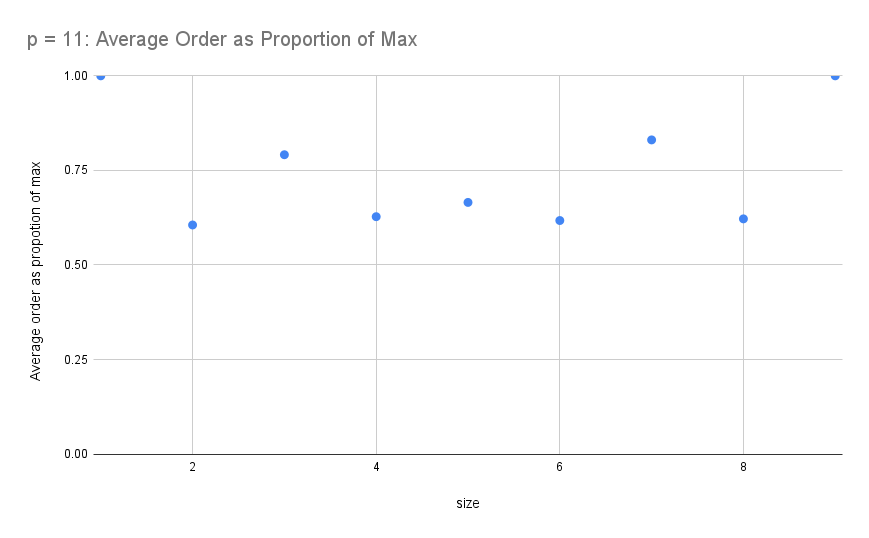
\includegraphics[width=1\textwidth]{p11_average.pdf}

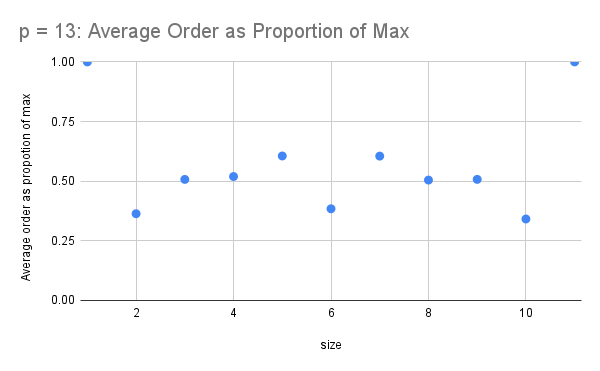
\includegraphics[width=1\textwidth]{p13_average.pdf}

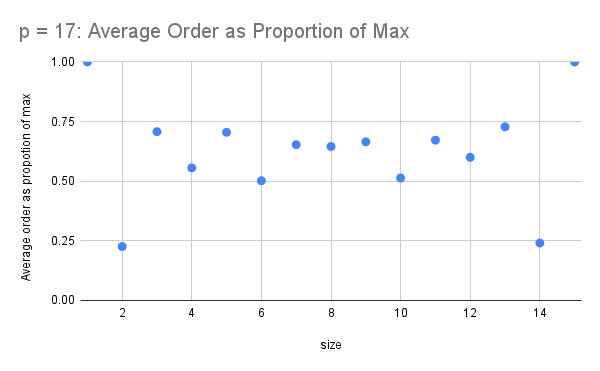
\includegraphics[width=1\textwidth]{p17_average.pdf}

The most obvious observation is that these graphs are nearly
perfectly symmetric. The average order for a size $s$
is the same as that for $p - 1 - s$.
This makes sense, since the order of a set of size
$s$ should have the same size as its inverse,
which has size $p - 1 - s$.

We can also see that when the size is 1 or $p - 2$,
the order is always maximized. However, this is also the most
restrictive category---there are only $2(p-1)$ such sets,
so we will exclude them from the rest of this analysis.

The jagged pattern of these graphs indicates that odd sizes
generally have higher orders than even sizes. At $p = 11$,
odd-size sets outperform even-size sets by by about 23\%;
at $p = 13$ by about 32\%; and at $p = 17$ by about 47\%.
Excluding sizes 2 and $p - 3$, we find that odd-size
sets outperform even-size sets by 18--22\% across the board.

While recording the data, we also noticed that many of the
sets have the same order. We will now look at the actual values
of the orders, and how many sets are associated with each order.

\includegraphics[width=1\textwidth]{p11_orders.pdf}

\includegraphics[width=1\textwidth]{p13_orders.pdf}

\includegraphics[width=1\textwidth]{p17_orders.pdf}

In all cases, we observed a strong linear relationship between
the order and the number of sets associated with that order.
We also observed a fascinating pattern---for every
$S \subseteq \zee_p'$ that we observed, its order
can be written as $n + 1$
for some $n \in \N$ with $n \mid 2^{p-1}-1$.
By Corollary 3.2, we can equivalently say that
$S^n = \zee_p'$.
Also note that for any $d \in \N$,
if $d \mid n$ and $S^d = \zee_p'$,
then $S^n = \zee_p'$.
Therefore, we need only ensure that
$S^{(2^{p-1}-1)/d} \neq \zee_p'$
for all prime divisors $d$ of $2^{p-1}-1$
to verify that the order of $S$ is $2^{p-1}$.

Ideally, we would select $p$ such that $2^{p-1}-1$ is prime.
However, this is impossible. Numbers of the form $2^n-1$
for some $n \in \N$ are known as Mersenne numbers,
and it is well-known that they can only be prime if $n$ is prime.
Since $p-1$ is even, excluding case where $p = 3$,
$2^{p-1}-1$ cannot be prime.
Therefore, we should select $p$
such that $2^{p-1}-1$ has as few divisors as possible.

We then propose the following steps to select $S$:
\begin{enumerate}
    \item Select a random set $S \in \zee_p'$ with an odd size
    $s$ such that $1 \leq s \leq p - 2$.
    \item For each prime divisor $d$ of $2^{p-1}-1$, compute
    $S^{(2^{p-1}-1)/d}$. If it is equal to $\zee_p'$, return to step 1.
    \item Proceed with set $S$.
\end{enumerate}
It may not be feasible to compute all prime divisors of
$2^{p-1}-1$. Say we are only able to find prime divisors
$d_1, d_2, \ldots, d_n$ with multiplicities $m_1, m_2, \ldots, m_n$.
Then, we can check $S^{(2^{p-1}-1) / d_i}$ for each $d_i$ as described
above, and we can also check $S^{d_1^{m_1}d_2^{m_2}\cdots d_n^{m_n}}$.
This will not ensure that the order of $S$ is $2^{p-1}$, but it will
eliminate many sets with lower orders.

In the final two sections, we will detail other concepts that we
explored, but did not find to be useful when developing the Diffie-Hellman
algorithm.

\section{Timular Arithmetic}

Let $x \in \N$.

\textbf{Definition 6.1.} Let $a, b \in \zee$.
Then, $a$ is \textit{similar to $b$ timulo} $x$,
denoted $a \sim b \tim x$,
if there exist $c_1, c_2, \ldots, c_r \in \zee$
with $c_1 \geq 0, c_2 \geq 0, \ldots, c_r \geq 0$
such that, for some $m_1, m_2, \ldots, m_r \in \zee$
\[a = c_1x^{m_1} + c_2x^{m_2} + \ldots + c_rx^{m_r}\]
and for some $n_1, n_2, \ldots, n_r \in \zee$,
\[b = c_1x^{n_1} + c_2x^{n_2} + \ldots + c_rx^{n_r}\]


\textbf{Lemma 6.1.} \textit{Similarity timulo $x$ is a
tolerance relation.}

First, we will show that it is reflexive. Let $a \in \zee$.
Then, $a = ax^0 \equiv ax^0 \equiv a \tim x$.

Symmetry is obvious, as similarity is defined without
regard to the order of $a$ and $b$. This proves the lemma.
$\blacksquare$


\textbf{Definition 6.2.} Let $a, b \in \zee$.
Then, $a$ is \textit{congruent to $b$ timulo} $x$, denoted
$a \equiv b \tim x$, if there exist some $d_1, d_2, \ldots, d_s \in \zee$
such that
\[a \sim d_1 \sim d_2 \sim \ldots \sim d_s \sim b \tim x\]

\textbf{Theorem 6.1.} \textit{Congruence timulo $x$ is an
equivalence relation.}

First, we will show that it is reflexive. Let $a \in \zee$.
By Lemma 6.1, $a \sim a \tim x$, so $a \equiv a \tim x$.

Next, we will show that it is symmetric. Let $a, b \in \zee$.
Let $d_1, d_2, \ldots, d_s \in \zee$ such that
\[a \sim d_1 \sim d_2 \sim \ldots \sim d_s \sim b \tim x\]
Then, by Lemma 6.1,
\[b \sim d_s \sim d_{s-1} \sim \ldots \sim d_1 \sim a \tim x\]
Therefore, $b \equiv a \tim x$.

Transitivity clearly follows from Definition 6.2. This proves the
theorem. $\blacksquare$

\textbf{Theorem 6.2.} \textit{Let $a \in \zee$.
Then, there exists a unique
$b \in \zee$ with $0 \leq b < x$
such that $a \equiv b \tim x$.}

We will first prove existence.
We can write $a$ as $mx + n$ for some
$m, n \in \zee$ with $m \geq 0$ and $0 \leq n < x$.
If $m = 0$, we are done, as $a < x$.
If $m = 0$, then we have $a' = mx + n$
with $a' \sim a \tim x$ and $a' < a$.
We can repeat this process indefinitely,
substituting $a'$ for $a$,
until $a' < x$.

Now, we will prove uniqueness. Let $b \in \zee$
with $0 \leq b < x$. If $b = 0$, then it is not
congruent to any other numbers, so we are done.
If $b > 0$,
we can rewrite it as $(b - 1) + 1$,
which shows us that the next greatest number congruent to
$b$ is $(b - 1) + x \geq x$.
This completes the proof of the theorem.
$\blacksquare$

\textbf{Definition 6.3.} Let $a \in \zee$.
$b \in \zee$ is the \textit{canonical form of $a$ timulo $x$}
if $0 \leq b < x$.

\textbf{Definition 6.4.} Let $a \in \zee$. The
\textit{congruence class of $a$ timulo $x$},
denoted $(a:x)$, is the set of all $b \in \zee$
such that $a \equiv b \tim x$.

\textbf{Lemma 6.2.} \textit{Let $a, a' \in \zee$ be
similar timulo $x$, and let $b \in \zee$. Then,
$(a + b) \sim (a' + b) \tim x$.}

Let $a = c_1x^{m_1} + c_2x^{m_2} + \ldots + c_rx^{m_r}$,
and let
$a' = c_1x^{n_1} + c_2x^{n_2} + \ldots + c_rx^{n_r}$.
Then,
\[\begin{split}
    a + b &= (c_1x^{m_1} + c_2x^{m_2} + \ldots + c_rx^{m_r}) + b \\
    &= c_1x^{m_1} + c_2x^{m_2} + \ldots + c_rx^{m_r} + bx^0 \\
    &\sim c_1x^{n_1} + c_2x^{n_2} + \ldots + c_rx^{n_r} + bx^0 \\
    &\sim (c_1x^{n_1} + c_2x^{n_2} + \ldots + c_rx^{n_r}) + b \\
    &\sim a' + b \tim x
\end{split}\]
This proves the lemma. $\blacksquare$

\textbf{Lemma 6.3.} \textit{Let $a, a' \in \zee$ be
congruent timulo $x$, and let $b \in \zee$. Then,
$a + b \equiv a' + b \tim x$.}

Let $d_1, d_2, \ldots, d_s \in \zee$
such that $a \sim d_1 \sim d_2 \sim \ldots \sim d_s \sim a' \tim x$.
Then, by Lemma 6.2,
\[(a + b) \sim (d_1 + b) \sim (d_2 + b) \sim \ldots
\sim (d_s + b) \sim (a' + b) \tim x\]
Therefore, $a + b \equiv a' + b \tim x$.
$\blacksquare$

\textbf{Lemma 6.4.} \textit{Let $a, a' \in \zee$ be
similar timulo $x$, and let $b \in \zee$. Then,
$ab \sim a'b \tim x$.}

Let $a = c_1x^{m_1} + c_2x^{m_2} + \ldots + c_rx^{m_r}$,
and let
$a' = c_1x^{n_1} + c_2x^{n_2} + \ldots + c_rx^{n_r}$.
Then,
\[\begin{split}
    ab &= (c_1x^{m_1} + c_2x^{m_2} + \ldots + c_rx^{m_r})b \\
    &= bc_1x^{m_1} + bc_2x^{m_2} + \ldots + bc_rx^{m_r} \\
    &\sim bc_1x^{n_1} + bc_2x^{n_2} + \ldots + bc_rx^{n_r} \\
    &\sim (c_1x^{n_1} + c_2x^{n_2} + \ldots + c_rx^{n_r})b \\
    &\sim a'b \tim x
\end{split}\]
This proves the lemma. $\blacksquare$

\textbf{Lemma 6.5.} \textit{Let $a, a' \in \zee$ be
congruent timulo $x$, and let $b \in \zee$. Then,
$ab \equiv a'b \tim x$.}

Let $d_1, d_2, \ldots, d_s \in \zee$
such that $a \sim d_1 \sim d_2 \sim \ldots \sim d_s \sim a' \tim x$.
Then, by Lemma 6.2,
\[ab \sim d_1b \sim d_2b \sim \ldots
\sim d_sb \sim a'b \tim x\]
Therefore, $ab \equiv a'b \tim x$.
$\blacksquare$

\textbf{Definition 6.5.} $T(x)$ denotes the set of all
congruence classes timulo $x$.

\textbf{Definition 6.6.} Let $a, b \in \zee$. Define
$(a:x) + (b:x)$ by $(a+b:x)$, and define $(a:x) \cdot (b:x)$
by $(ab:x)$.

\textbf{Theorem 6.3.} \textit{Let $A, B \in \zee_p'$.
Then, $\beta(A \oplus_k B) \equiv \beta(A) + \beta(B) \tim 2^{p-1}$.}

This theorem is an alternate formulation of Theorem 3.1 and the proof
would be nearly identical, so it is not detailed here.

\section{$\oplus_k$ over $\N$}

\textbf{Definition 7.1.} Define $R \subseteq \N$ by
\[R = \{n \in \N \mid k \nmid n\}\]
Let $R = \{r_1, r_2, r_3, \ldots\}$ with $r_1 < r_2 < r_3 < \ldots$.

\textbf{Definition 7.2.} Let $n \in \N$ and let $A \in \mathcal{P}_f(\N)$.
For all $i \in \zee$
with $i \geq 0$, let $z_i = 0$ if $nk^i \not\in A$,
and let $z_i = 1$ if $nk^i \in A$.
Define $\beta': \N \times \mathcal{P}(\N) \rightarrow \N$
by
\[\beta'(n, A) = \sum_{i = 0}^\infty z_i \cdot 2^{i}\]
This is a more general form of $\beta$ from Definition 3.2.
For $A \in \zee_p'$, $\beta(A)$ is generally
the same as $\beta'(1, A)$.

\textbf{Definition 7.3.} Let
$p_1, p_2, p_3, \ldots \in \N$ denote the primes in increasing
order---that is, $p_1 = 2$, $p_2 = 3$, $p_3 = 5$, etc.
Let $A \in \mathcal{P}_f(\N)$.
Then, define $\alpha: \mathcal{P}(\N) \rightarrow \N$ by
\[\alpha(A) = \prod_{i=1}^\infty p_i^{\beta'(r_i, A)}\]
We will consider an example. Suppose $k = 4$, and let
$A = \{1, 3, 4, 9, 16, 48\}$.
\begin{itemize}
    \item Consider $i = 1$. We are interested in $r_1 = 1$.
    $r_1k^0 = 1 \in A$,
    $r_1k^1 = 4 \in A$, and $r_1k^2 = 16 \in A$.
    Therefore,
    \[\beta'(r_1, A) = \beta'(1, A) = \text{0b111} = 7\]
    \item Consider $i = 2$. We are interested in $r_2 = 2$.
    Since there is no $n \in \N$ for which $2k^n \in A$,
    we find
    \[\beta'(r_2, A) = \beta'(2, A) = 0\]
    \item Consider $i = 3$. We are interested in $r_3 = 3$.
    $r_3k^0 = 3 \in A$ and $r_3k^2 = 48 \in A$.
    Therefore,
    \[\beta'(r_3, A) = \beta'(3, A) = \text{0b101} = 5\]
    \item Consider $i = 7$. We are interested in $r_7 = 9$.
    $r_7k^0 = 9 \in A$. Therefore,
    \[\beta'(r_7, A) = \beta'(9, A) = \text{0b1} = 1\]
\end{itemize}
Therefore,
\[\begin{split}
    \alpha(A) &= p_1^7 \cdot p_3^5 \cdot p_7^1 \\
    &= 2^7 \cdot 5^5 \cdot 17 \\
    &= 6800000
\end{split}\]
We claim that $\alpha$ is a bijection.

\textbf{Theorem 7.1.} \textit{Let $A, B \in \mathcal{P}_f(\N)$.
Then, $\alpha(A \oplus_k B) = \alpha(A) \cdot \alpha(B)$.}

Let $i \in \N$.
Recall $\gamma$ from Definition 3.3.
Since we are considering the natural numbers
instead of a modular field, we can replace the $L$ function
with multiplication by 2, to find that
$\beta'(r_i, A) + \beta'(r_i, B) = \beta'(r_i, A \oplus_k B)$.

Note that for any set $S \in \mathcal{P}_f(\N)$,
any number represented by a bit in
$\beta'(r_i, S)$ can be written in the form $r_ik^n$
for some $n \in \zee$ with $n \geq 0$, and any number
not represented there cannot be written in this form.
Therefore, we can consider each $p_i$ separately,
as they create isolated partitions of the set.

We will now consider the product of $\alpha(A)$ and $\alpha(B)$.
\[\begin{split}
    \alpha(A) \cdot \alpha(B) &=
    \prod_{i=1}^\infty p_i^{\beta'(r_i, A)}
    \cdot \prod_{i=1}^\infty p_i^{\beta'(r_i, B)} \\
    &= \prod_{i=1}^\infty p_i^{\beta'(r_i, A) + \beta'(r_i, B)} \\
    &= \prod_{i=1}^\infty p_i^{\beta'(r_i, A \oplus_k B)} \\
    &= \alpha(A \oplus_k B)
\end{split}\]
This completes the proof of the theorem. $\blacksquare$


\end{document}
